\documentclass[11pt]{article}

\usepackage[margin=1in]{geometry}
\usepackage{tikz}
\usepackage{amsmath}
\usepackage{amssymb}
\usepackage{outlines}
\usepackage{algorithm}
\usepackage{algpseudocode}

\begin{document}

\begin{flushright}
Andrew Leverentz
\end{flushright}

We begin by considering a taxonomy of hierarchical clustering algorithms (Figure \ref{fig:taxonomy}).
A \emph{hierarchical clustering} is a tree in which the leaves correspond to individual points in the input dataset, and each internal node corresponds to the subset of the data corresponding to the node's descendant leaves.
Then, a \emph{hierarchical clustering algorithm} is merely an algorithm which takes as input an unlabeled dataset and outputs a hierarchical clustering.
When constructing a hierarchical clustering, the goal is typically to find a nested set of splits which separate highly ``dissimilar'' points toward the top of the tree, and which separate highly ``similar'' points much closer to the leaves.

\begin{figure}[h]
\centering
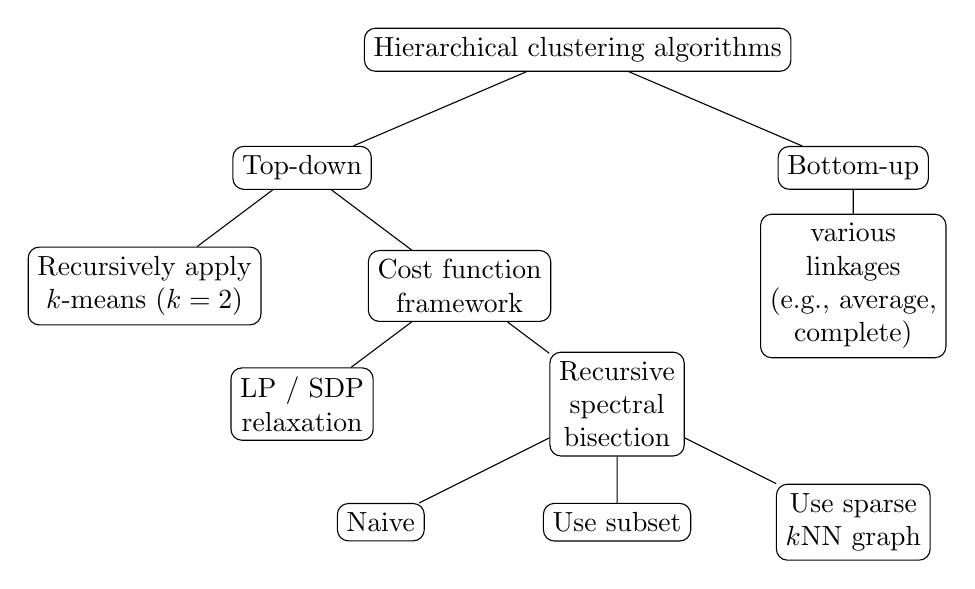
\begin{tikzpicture}[
  every node/.style = {
    shape=rectangle,
    rounded corners,
    draw,
    align=center
  },
  level 1/.style={sibling distance=7cm},
  level 2/.style={sibling distance=4cm},
  level 3/.style={sibling distance=4cm},
  level 4/.style={sibling distance=3cm},
  level 5/.style={sibling distance=3cm},]
  \node {Hierarchical clustering algorithms}
    child { node {Top-down}
      child { node {Recursively apply \\ $k$-means ($k = 2$)} }
      child { node {Cost function \\ framework}
        child { node {LP / SDP \\ relaxation} }
        child { node {Recursive \\ spectral \\ bisection}
          child { node {Naive} }
          child { node {Use subset} }
          child { node {Use sparse \\ $k$NN graph} }
        }
      }
    }
    child { node {Bottom-up}
      child { node {various \\ linkages \\ (e.g., average, \\ complete)}}
    };
\end{tikzpicture}
\caption{Taxonomy of hierarchical clustering algorithms}
\label{fig:taxonomy}
\end{figure}

A hierarchical clustering algorithm may be either bottom-up or top-down.
A \emph{bottom-up} algorithm starts by putting each observation into its own cluster, and it repeatedly combines them according to some criterion (e.g., single linkage, average linkage, and so on).
This approach is ``bottom-up'' because we start at the leaves and work our way toward the root by combining clusters.
A \emph{top-down} algorithm starts by putting all observations into a single cluster, and it repeatedly divides each node according to some criterion.
In this setting, we start at the root and work our way toward the leaves.

One approach to top-down clustering is to recursively apply a simple binary splitting algorithm (such as $k$-means with $k=2$).
However, one major downside to this approach is that it cannot handle clusters with highly irregular boundaries, and in such cases it may end up producing splits which place very similar points into different high-level clusters.

Dasgupta [2016] defines a cost-function framework for hierarchical clustering.
Any algorithm which minimizes (or approximately minimizes) the given cost function belongs to this class.
One particular subset of these algorithms are those which recursively split clusters into two, while attempting to minimize the RatioCut (**TODO: confirm terminology) at each stage.

Several authors (**TODO: citations) have proposed optimizing the via relaxations (LP or SDP).
Unfortunately, these algorithms have runtimes of $\Omega(n^3)$ and therefore suffer from the same scaling limitations as most bottom-up clustering algorithms.

Recursive spectral bisection (i.e., repeated application of 2-way spectral clustering) involves computing a particular eigenvector (the ``Fiedler vector'') of the graph Laplacian corresponding to the pairwise similarity matrix of the dataset.
This approach is known to approximately minimize the RatioCut (**TODO: confirm terminology) of the similarity graph.
However, a naive implentation, using a dense similarity matrix and standard eigenvector computations, once again has a runtime of $\Omega(n^3)$.

Several modifications to recursive spectral bisection can improve its performance:
\begin{enumerate}
    \item Applying spectral clustering to the result of $k$-means clustering (where $k \ll n$)
    \item Using a randomly selected subset
    \item Constructing a sparse $k$-nearest neighbor ($k$NN) graph prior to performing spectral clustering
\end{enumerate}

For now, we focus on the third option. 
Using Fast Nearest Neighbor data structures (such as metric trees or random projection trees), we can efficiently compute a sparse $k$NN graph.
From this sparse $k$NN graph, we construct a sparse similarity matrix and then apply spectral clustering.

There are several important considerations involved in this process:
\begin{itemize}
    \item Converting a distance matrix to a similarity matrix involves a scaling parameter which needs to be selected according to an adaptive criterion.
    \item The parameter $k$ should grow as a function of $n$ (otherwise the sparse similarity graph will contain a large number of disconnected components), but if it grows too quickly, the algorithm will no longer scale sub-quadratically.  (Ideally, $k$ should be sublinear in the dataset size $n$; for example, $k \in O(\log n)$.)
    \item The algorithm should handle disconnected components in a sensible way (for example, by partitioning them such that the number of observations assigned to each side of a split is roughly balanced).
    \item Linear algebra operations (in particular, eigenvalue/eigenvector computations) must be implemented in a way that takes advantage of the sparsity of the similarity matrix.
\end{itemize}

Next, we outline our implementation of top-down spectral hierarchical clustering.

\newcommand{\algparbox}[2]{\parbox[t]{\dimexpr\linewidth-(\algorithmicindent * #1)\relax}{%
  \setlength{\hangindent}{\algorithmicindent}%
  #2}}

\begin{algorithm}
\caption{Spectral hierarchical clustering (main routine)}
\begin{algorithmic}
\Function{Clustering}{dataset $S$, integer $k$}
    \State $d \gets \Call{GetDistances}{S, k}$
    \State $c \gets \Call{GetConnectedComponents}{d}$
    \State \Return $\Call{ClusterMultipleComponents}{d, c}$
\EndFunction
\end{algorithmic}
\end{algorithm}

\begin{algorithm}
\caption{Distance and connected-component computations}
\begin{algorithmic}
\Function{GetDistances}{dataset $S$, integer $k$}
  \State For each observation $\mathbf x \in S$, compute the $k$ nearest neighbors of $\mathbf x$ within $S$.
  \State (This can be done using metric trees, for example.)
  \State Construct a sparse matrix $d$ containing the distances to each of the $k$ nearest neighbors.
  \State If the resulting matrix is not symmetric, add entries until it becomes symmetric.
  \State \Return $d$
\EndFunction

\vspace{1em}
\noindent
\emph{Implementation note:} We must be careful to distinguish between elements of the distance matrix which are $0$ because the corresponding entry does not appear in the nearest-neighbor graph, and elements which are $0$ because the pairwise distance is truly $0$.
To do this, we can use a special value, such as \texttt{NaN} to indicate that an entry corresponds to a true distance of $0$.
Later, when we compute the similarity matrix, we will interpret a missing entry as a distance of $+\infty$, corresponding to a similarity of $0$, and we will interpret an entry of \texttt{NaN} as a distance of $0$, corresponding to a similarity of $1$.

\vspace{1em}
\Function{GetConnectedComponents}{sparse distance matrix $d$}
  \State $i \gets 0$
  \State $c \gets$ vector of $n$ zeros
  \While {unvisited vertices remain}
    \State Perform breadth-first search starting from an unvisited vertex
    \State For each vertex $v$ visited in this round, set $c[v] \gets i$
    \State $i \gets i + 1$
  \EndWhile
  \State \Return $c$
\EndFunction
\end{algorithmic}
\end{algorithm}

\begin{algorithm}
\caption{Clustering for one or more components}
\begin{algorithmic}
\Function{ClusterMultipleComponents(}{}
  \State
    \begin{tabular}{ll}
    \hspace{4em}
    & dataset $S$, \\
    & sparse distance matrix $d$, \\
    & vector of connected components $c$)
    \end{tabular}
  \If {$\Call{NumComponents}{c} = 1$}
    \State \Return $\Call{ClusterSingleComponent}{S, d}$
  \Else
    \State Define $S_\ell$, $S_r$, $d_\ell$, $d_r$, $c_\ell$, and $c_r$ as follows:
    \State Find the largest 2 components in $c$
    \State Put all observations from the largest component into $S_\ell$
    \State Put all observations from the second-largest component into $S_r$
    \For {each remaining component}
      \State \algparbox{4}{Put all observations from the current component into either $S_\ell$ or $S_r$, whichever is currently smaller}
    \EndFor
    \State Update $d_\ell$, $d_r$, $c_\ell$, and $c_r$ to be consistent with $S_\ell$ and $S_r$
    \State $T_\ell \gets \Call{ClusterMultipleComponents}{S_\ell, d_\ell, c_\ell}$
    \State $T_r \gets \Call{ClusterMultipleComponents}{S_r, d_r, c_r}$
    \State \Return a node with children $T_\ell$ and $T_r$
  \EndIf
\EndFunction

\vspace{1em}
\Function{ClusterSingleComponent}{dataset $S$, sparse distance matrix $d$}
  \If {$\Call{NumObservations}{S} \leq $ max leaf size}
    \State \Return a single leaf
  \Else
    \State $(S_\ell, S_r) \gets \Call{Partition}{S, d}$
    \State $T_\ell \gets \Call{Clustering}{S_\ell, k}$
    \State $T_r \gets \Call{Clustering}{S_r, k}$
    \State \Return a node with children $T_\ell$ and $T_r$
  \EndIf
\EndFunction
\end{algorithmic}
\end{algorithm}

\begin{algorithm}
\caption{Split a node into a 2-way partition}
\begin{algorithmic}
\Function{Partition}{dataset $S$, sparse distance matrix $d$}
  \If {$\Call{NumObservations}{d} = 2$}
    \State \algparbox{3}{\Return a partition in which the first observation is sent to the left, and the second observation is sent to the right}
  \Else
    \State $s \gets \Call{GetSimilarity}{d}$
    \State $r \gets \Call{SumByRow}{s}$
    \State $L \gets \Call{Diagonal}{r} - s$
    \State $v \gets \Call{GetFiedlerVector}{L}$
    \State \algparbox{3}{\Return a partition where observations corresponding to positive entries of $v$ are sent to the left, and all others are sent to the right} 
  \EndIf
\EndFunction
\end{algorithmic}
\end{algorithm}

\begin{algorithm}
\caption{Convert a sparse distance matrix into a sparse similarity matrix}
\begin{algorithmic}
\Function{GetSimilarity}{sparse distance matrix $d$}
  \State $m \gets $ median value of non-missing entries of $d$ (computed via quickselect)
  \State $\sigma \gets m (2 \log(1/\alpha))^{-1/2}$
  \State Here, $\alpha$ is a user-specified parameter, with a default value of $0.8$.
  \State $s \gets $ empty sparse matrix with the same dimensions as $d$
  \For {each entry $d_{i,j}$ in the sparse matrix $d$}
    \If {$d_{i,j} = \texttt{NaN}$}
      \State $s_{i,j} \gets 1$
    \Else
      \State $s_{i,j} \gets \exp(-d_{i,j}^2 / (2 \sigma^2))$
    \EndIf
  \EndFor
  \State Convert $s$ to Compressed Sparse Row (CSR) format
  \State \Return $s$
\EndFunction

\vspace{1em}
\noindent
\emph{Note:} The adaptive selection of the scaling parameter $\sigma$ guarantees that whenever $d_{i,j} = m$, we have $s_{i,j} = \alpha$.
\end{algorithmic}
\end{algorithm}

\begin{algorithm}
\caption{Compute the Fiedler vector of a Laplacian matrix}
\begin{algorithmic}
\Function{GetFiedlerVector}{sparse matrix $A$}
  \If {$A$ is sufficienly small (say, $10 \times 10$ or smaller)}
    \State Compute the full eigendecomposition of $A$
    \State \Return the eigenvector corresponding to the second-smallest eigenvalue
  \Else
    \State $u \gets $ a constant unit vector
    \State $x \gets $ random vector perpendicular to $u$
    \For {a small, fixed number of iterations}
      \State $x \gets \Call{SolveConjugateGradient}{A, x}$
      \State \emph{Note:} this approximates $x \gets A^{-1} x$ (inverse power iteration)
      \State Make $x$ perpendicular to $u$ by subtracting its projection
      \State Renormalize $x$ to be a unit vector
    \EndFor
    \State \Return $x$
  \EndIf
\EndFunction

\vspace{1em}
\Function{SolveConjugateGradient}{sparse matrix $A$, vector $b$}
  \State Perform a small, fixed number of iterations of the conjugate gradient method
  \State This involves a fixed number of sparse matrix-vector multiplications
  \State \Return the resulting vector
\EndFunction
\end{algorithmic}
\end{algorithm}

% \begin{algorithm}
% \caption{XYZ}
% \begin{algorithmic}
% \Function{XYZ}{XYZ}
%   \State XYZ
% \EndFunction
% \end{algorithmic}
% \end{algorithm}

\clearpage
\paragraph{Rough algorithmic analysis:}
I think the distance computation is the main bottleneck within each recursive call, and it can be done in $O(k n \log n)$ time with metric trees.
Then, if the splits are always likely to be reasonably well-balanced, I think the overall runtime should be $O(k n \log^2 n)$.

\paragraph{A few more things to consider...}
\begin{itemize}
\item Should we avoid re-computing nearest neighbors in each recursive call?
(As a side effect, this would also allow the algorithm to operate directly on pre-computed sparse graphs.)
It's not immediately clear how much would this affect the results, if at all.
\item I'm currently using a very naive implementation of \textsc{GetFiedlerVector}.
We may want to add an adaptive convergence condition (rather than a fixed number of iterations) and perhaps some kind of sparse matrix preconditioning.
The current implementation may not always get sufficiently close to convergence.
\end{itemize}
\end{document}